\documentclass[10pt]{article}
\usepackage[polish]{babel}
\usepackage[utf8]{inputenc}
\usepackage[T1]{fontenc}
\usepackage{amsmath}
\usepackage{amsfonts}
\usepackage{amssymb}
\usepackage[version=4]{mhchem}
\usepackage{stmaryrd}
\usepackage{graphicx}
\usepackage[export]{adjustbox}
\graphicspath{ {./images/} }

\title{GIMNAZJUM }

\author{}
\date{}


\begin{document}
\maketitle
\begin{enumerate}
  \item Dany jest trapez \(A B C D\) o podstawach \(A B\) i \(C D\), w którym kąty \(B A D\) i \(A B C\) mają po \(60^{\circ}\) oraz \(C D<B C\). Na boku \(B C\) tego trapezu wybrano taki punkt \(E\), że \(E B=C D\). Wykaż, że odcinki \(B D\) i \(A E\) są równej długości.\\
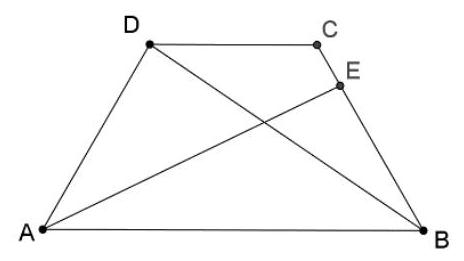
\includegraphics[max width=\textwidth, center]{2024_11_21_913e907bded18b80a017g-1(1)}
  \item Uzasadnij, że liczba \(\frac{6+6^{2}+6^{3}+\cdots+6^{2016}}{7}\) jest liczbą całkowitą.
  \item Udowodnij, że dla dowolnej liczby naturalne \(n\) co najmniej jedna z liczb: \(n^{3}-n\); \(n^{3}+n\) jest podzielna przez 10. Kiedy obie te liczby są jednocześnie podzielne przez 10?
\end{enumerate}

\section*{LICEUM}
\begin{enumerate}
  \item Wykaż, że w trójkącie o bokach \(a, b, c\) i wysokościach odpowiednio \(h_{a}, h_{b}, h_{c}\) zachodzi równość
\end{enumerate}

\[
(a+b+c) \cdot\left(\frac{1}{a}+\frac{1}{b}+\frac{1}{c}\right)=\left(h_{a}+h_{b}+h_{c}\right) \cdot\left(\frac{1}{h_{a}}+\frac{1}{h_{b}}+\frac{1}{h_{c}}\right)
\]

\begin{enumerate}
  \setcounter{enumi}{1}
  \item Dwusieczne kątów \(B A C\) i \(A B C\) trójkąta \(A B C\) przecinają przeciwległe boki tego trójkąta odpowiednio w punktach \(D\) i \(E\). Wiedząc, że \(A E+B D=A B\), wyznacz miarę kąta ACB.
  \item Cyfry rozwinięcia dziesiętnego liczb \(2^{2016}\) i \(5^{2016}\) wypisano kolejno jedna za drugą. Oblicz, ile zapisano\\
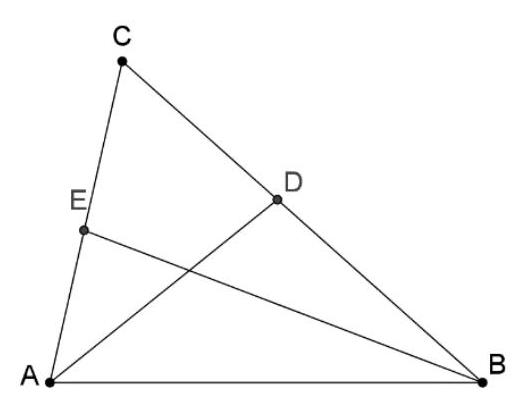
\includegraphics[max width=\textwidth, center]{2024_11_21_913e907bded18b80a017g-1}\\
cyfr.
\end{enumerate}

\end{document}